\title{Algebraic graph calculus}



\newcommand{\1}{\mathbf{1}}
\newcommand{\R}{\mathbf{R}}




We describe a graph-theoretic analogue of vector calculus.  The linear
operators of vector calculus (gradient, divergence, laplacian) correspond to
the matrices naturally associated to graphs (incidence matrix, adjacency
matrix).  This analogy is useful for formalizing the discretization of some
problems in image and surface processing that are often defined in a continuous
setting.




\section{Reminder of vector calculus}


Vector calculus deals with functions and vector fields defined in $\R^3$.



\subsection{Functions and vector fields}


A \emph{function} (or \emph{scalar field}) is a map $u:\R^3\to\R$.
A \emph{vector field} is a map $\mathbf{v}:\R^3\to\R^3$.
Vector fields are written in bold.



Let us fix some typical names for the coordinates.
The coordinates of a point in $\R^3$ are written as $(x,y,z)$.
If $\mathbf{v}$ is a vector field, then $\mathbf{v}=(a,b,c)$ where $a$, $b$
and $c$ are three scalar fields called the components of $\mathbf{v}$.
We denote the partial derivatives of a function using subindices, for
example $a_y:=\frac{\partial a}{\partial y}$.


\subsection{Differential operators}


The \emph{gradient} of a function $u$ is a vector field $\nabla u$ defined
by
\[
\nabla u = \left(
u_x\ ,\ u_y\ ,\ u_z
%\frac{\partial u}{\partial x},
%\frac{\partial u}{\partial y},
%\frac{\partial u}{\partial z}
\right)
\]




The \emph{divergence} of a vector field $\mathbf{u}=(a,b,c)$ is a scalar
field $\mathrm{div}(\mathbf{u})$ defined by
\[
\mathrm{div}(\mathbf{u}) =
a_x + b_y + c_z
\]
%\frac{\partial a}{\partial x}+
%\frac{\partial b}{\partial y}+
%\frac{\partial c}{\partial z}




The \emph{curl} of a vector field $\mathbf{u}=(a,b,c)$ is another vector
field $\mathrm{curl}(\mathbf{u})$ defined by
\[
\mathrm{curl}(\mathbf{u}) =
\left(
c_y - b_z\ ,\ a_z - c_x\ ,\ b_x - a_y
\right)
\]
%\frac{\partial c}{\partial y} - \frac{\partial b}{\partial z},\ \ 
%\frac{\partial c}{\partial y} - \frac{\partial b}{\partial z},\ \ 
%\frac{\partial c}{\partial y} - \frac{\partial b}{\partial z},



Finally, the \emph{laplacian} of a scalar field $u$ is the scalar field
$\Delta u$ defined by
\[
\Delta u = u_{xx} + u_{yy} + u_{zz}.
\]




Notice that, except for the curl, all these operations can be defined in
$\R^N$.  However, the curl is specific to three dimensions.  There is a
similar operator in two dimensions, which we call also the curl and computes
a scalar field $\mathrm{curl}(\mathbf{u})$ from a vector field
$\mathbf{u}=(a,b):\R^2\to\R^2$
\[
\mathrm{curl}(\mathbf{u}) = b_x - a_y
\]
Notice that it is the last component of the 3D curl.


The curl is also defined in dimension 7.
Let~$\mathbf{u}=(u^1,\ldots,u^7)$ be a vector field in~$\R^7$, then
\[
%\renewcommand*{\arraystretch}{1.5}
\def\curlco#1#2#3#4#5#6{%
{u^{#1}}_{#2}-{u^{#2}}_{#1}+
{u^{#3}}_{#4}-{u^{#4}}_{#3}+
{u^{#5}}_{#6}-{u^{#6}}_{#5}%
}
\mathrm{curl}(\mathbf{u}) =
\left(
	\begin{matrix}
		\curlco{2}{4}{3}{7}{5}{6} \\
		\curlco{3}{5}{4}{1}{6}{7} \\
		\curlco{4}{6}{5}{2}{7}{1} \\
		\curlco{5}{7}{6}{3}{1}{2} \\
		\curlco{6}{1}{7}{4}{2}{3} \\
		\curlco{7}{2}{1}{5}{3}{4} \\
		\curlco{1}{3}{2}{6}{4}{5} \\
	\end{matrix}
\right)
\]
where a sub-index~$i$ denotes a partial derivative in the $i$-th dimension
of~$\R^7$.  And analogously we can define the 6-dimensional curl by taking the last component (resulting in a scalar field).


\subsection{Differential identities and properties}


The most important identity is $\Delta u = \mathrm{div}(\mathrm{grad}(u))$,
that can be used also as the definition of $\Delta$.



Other identities involving the curl are
$\mathrm{curl}(\nabla u)=0$ and
$\mathrm{div}(\mathrm{curl}(\mathbf{u}))=0$.



The functions $u$ such that $\nabla u=0$ on $\R^3$ are the constants.



The vector fields $\mathbf{v}$ such that $\mathrm{curl}(\mathbf{v})=0$ are
called \emph{conservative}, \emph{irrotational} or \emph{integrable}.
They are of the form $\mathbf{v}=\nabla u$ for some function $u$ called the
\emph{potential} of $\mathbf{v}$.




The vector fields $\mathbf{v}$ such that $\mathrm{div}(\mathbf{v})=0$ are called
\emph{divergence-free}, \emph{volume-preserving}, \emph{solenoidal} or
\emph{incompressible}.
They are of the form $\mathbf{v}=\mathrm{curl}(\mathbf{u})$ for some vector
field $\mathbf{u}$ called the
\emph{vector potential} of $\mathbf{v}$.



The scalar fields $u$ such that $\Delta u=0$ are called
\emph{harmonic functions}.



The following identities are immediate applications of the product rule for
derivatives:
\[ \nabla(fg) = f\nabla g + g\nabla f \]
\[ \mathrm{div}(f\mathbf{g}) = f\mathrm{div}(\mathbf{g}) + \mathbf{g}\cdot\nabla f \]


\subsection{Integral calculus}


The divergence theorem:
\[
\int_\Omega \mathrm{div}(\mathbf{g}) =
\int_{\partial\Omega}\mathbf{g}\cdot\mathbf{ds}
\]



Combining the divergence theorem with the product rule we obtain the
integration by parts formula.
\[
\int_{\partial\Omega} f\mathbf{g}\cdot\mathbf{ds} =
\int_\Omega
f\mathrm{div}(\mathbf{g})
+
\int_\Omega
\mathbf{g}\cdot\nabla f
\]



Thus, if at least one of the two functions vanishes on the boundary of
$\Omega$
\[
0=
\int_\Omega
f\mathrm{div}(\mathbf{g})
+
\int_\Omega
\mathbf{g}\cdot\nabla f
\]
or, in another notation
\[
\left\langle
f, \mathrm{div}(\mathbf{g})
\right\rangle
=
\left\langle
-\nabla f, \mathbf{g}
\right\rangle
\]
thus that the operators $\mathrm{div}$ and $-\nabla$ are adjoint to each
other.  Integrating by parts twice we obtain that the operator $\Delta$ is
self-adjoint.


\section{Graphs and their matrices}


A \emph{graph} is $G=(V,E)$ where $V$ is a set called the
\emph{vertices} of $G$, and $E$ is a subset of $V\times V$ called the
\emph{edges} of $G$.



We assume always that the set $V$ is finite, and its elements are numbered
from $1$ to $n$.  Thus, the set $E$ is also finite (the cardinal is at most
$n^2$) and we assume that the elements of $E$ are numbered from $1$ to $m$.


\begin{tabular}{ll}
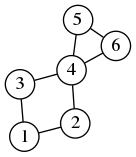
\includegraphics{graph1.png} &
%SCRIPT echo 'graph {1--2--4--5--6--4--3--1}' | neato -Tpng > graph1.png
$\begin{cases}
V  & = \{1,2,3,4,5,6\} \\
E  & = \{ \{1,2\},\{1,3\},\{2,4\},\{3,4\},\{4,5\},\{5,6\},\{4,6\} \}
\end{cases}$
\end{tabular}


\subsection{The adjacency list}


Given a graph of $n$ vertices and $m$ edges,
the adjacency list is a matrix
of $m$ rows and $2$ columns that contains the pairs of vertices connected by
each edge.  The entries of this matrix are integers on the set
$\{1,\ldots,n\}$. Thus, if the $k$-th row is $(i,j)$, this means that edge
$k$ connects vertices $i$ to $j$.

\begin{tabular}{ll}
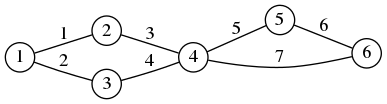
\includegraphics{graph2.png} &
%SCRIPT echo 'graph {
%SCRIPT 1--2 [label="1"]
%SCRIPT 1--3 [label="2"]
%SCRIPT 2--4 [label="3"]
%SCRIPT 3--4 [label="4"]
%SCRIPT 4--5 [label="5"]
%SCRIPT 5--6 [label="6"]
%SCRIPT 4--6 [label="7"]
%SCRIPT }' | dot -Tpng > graph2.png
\begin{equation*}
	\textrm{adjacency list} =
	\begin{pmatrix}
		1 & 2 \\
		1 & 3 \\
		2 & 4 \\
		3 & 4 \\
		4 & 5 \\
		5 & 6 \\
		4 & 6 \\
	\end{pmatrix}
\end{equation*}
\end{tabular}


The adjacency list is a very efficient representation for sparse graphs (where
the number of edges is proportional to the number of vertices).
However, it is not very interesting from the algebraic point of view.
We will see in the following three other matrices that have a very rich
algebraic interpretation.


\subsection{The adjacency matrix $A$}


Given a graph of $n$ vertices and $m$ edges,
the adjacency matrix is a square matrix $A=a_{ij}$ of size $n\times n$.
The entries of $A$ are zeros and ones, with $a_{ij}=1$ if there is an edge
from $i$ to $j$ and $a_{ij}=0$ otherwise.

$$
A =
\begin{array}{l|lllllll}
	V\backslash V
	  & 1 & 2 & 3 & 4 & 5 & 6 \\
	\hline
	1 & 0 & 1 & 1 & 0 & 0 & 0 \\
	2 & 1 & 0 & 0 & 1 & 0 & 0 \\
	3 & 1 & 0 & 0 & 1 & 0 & 0 \\
	4 & 0 & 1 & 1 & 0 & 1 & 1 \\
	5 & 0 & 0 & 0 & 1 & 0 & 1 \\
	6 & 0 & 0 & 0 & 1 & 1 & 0 \\
\end{array}
$$

Notice that this matrix has somewhat less information than the adjacency
list, because the ordering of the edges is lost.  Thus, there is a unique way
to compute the adjacency matrix from the list, but many $m!$ different ways
to get the list from the matrix.  We can chose an arbitrary canonical
ordering of the edges (for example, in lexicographic order).


\subsection{The Laplacian matrix $L$}


Let $A$ be the adjacency matrix of a graph $G$.
If we sum the values of all the elements of the $i$-th row, we obtain the
number of edges going out of vertex $i$ (called the degree of the edge).
Let us put the vector with all the degrees in the diagonal of a matrix $D$; in
octave/matlab notation $\mathtt{D=diag(sum(A))}$.
The Laplacian matrix of $G$ is defined as
\[
L = A - \mathtt{diag}(\mathtt{sum}(A))
\]
In the typical case where $A$ is symmetric with 0 on the diagonal, the matrix
L is the same as A with minus the degree of each vertex on the diagonal
entries.

$$
L =
\begin{array}{l|lllllll}
	V\backslash V
	  & 1 & 2 & 3 & 4 & 5 & 6 \\
	\hline
	1 &-2 & 1 & 1 & 0 & 0 & 0 \\
	2 & 1 &-2 & 0 & 1 & 0 & 0 \\
	3 & 1 & 0 &-2 & 1 & 0 & 0 \\
	4 & 0 & 1 & 1 &-4 & 1 & 1 \\
	5 & 0 & 0 & 0 & 1 &-2 & 1 \\
	6 & 0 & 0 & 0 & 1 & 1 &-2 \\
\end{array}
$$


\subsection{The incidence matrix $B$}


Given a graph of $n$ vertices and $m$ edges,
the incidence matrix is a rectangular matrix $B=b_{ij}$ of $m$ rows and $n$
columns.  The entries of $B$ are zeros, ones and minus ones given by the
edges of the graph: if the $k$-th edge goes from $i$ to $j$, then, on the
$k$th row there are values $-1$ and $1$ on positions $i$ and $j$
respectively; there are zeros everywhere else.

$$
B =
\begin{array}{l|lllllll}
	E\backslash V
	  & 1 & 2 & 3 & 4 & 5 & 6 \\
	\hline
	1 &-1 & 1 & 0 & 0 & 0 & 0 \\
	2 &-1 & 0 & 1 & 0 & 0 & 0 \\
	3 & 0 &-1 & 0 & 1 & 0 & 0 \\
	4 & 0 & 0 &-1 & 1 & 0 & 0 \\
	5 & 0 & 0 & 0 &-1 & 1 & 0 \\
	6 & 0 & 0 & 0 & 0 &-1 & 1 \\
	7 & 0 & 0 & 0 &-1 & 0 & 1 \\
\end{array}
$$



Notice that the incidence matrix contains the same information as the
adjacency list (including the order of the edges).



There is an interesting relationship between the incidence matrix and the
Laplacian matrix, that can be checked algebraically:
\[
L = -B^TB
\]
This identity is the discrete analogue of $\Delta=\mathrm{div\ grad}$,
as we will explain below.



\subsection{The unsigned incidence matrix $C$}


The incidence matrix $B$ defined above is signed, on each row there are two
non-zero entries whose values are $-1$ and $1$.  Thus the sum of any row is
zero.
We can write the matrix $B$ as $B=B_1-B_0$, where the matrices
$B_0$ and $B_1$ have only zeros and ones, with a single non-zero entry per
row.



It will be useful later to consider the \emph{unsigned incidence matrix}
$C$, defined as $C=\frac{1}{2}(B_0 + B_1)$, or equivalently
$C=\frac{1}{2}|B|$.  The rows of the matrix $C$ sum to one.



The following relations are immediate to verify
\[
A = 2C^TC-B^TB/2
\]
\[
\mathrm{deg} = 2C^TC+B^TB/2
\]
where $\mathrm{deg}$ is an $n\times n$ diagonal matrix, whose values are the
degrees of each vertex.



\section{Vector calculus on graphs}


Most of the constructions that we have described on the vector calculus
reminder above have a direct correspondence in the case of graphs.


\subsection{Analogies}


The correspondence between vector calculus and graph theory is laid out in
the following table.
%Table~\ref{tab:analogy}.
The main idea is that scalar fields correspond to
functions defined on vertices, and vector fields correspond to functions
defined on edges.

\begin{table}[ht]
\begin{tabular}{l|l}
	
		Vector calculus&
		Graph theory\\\hline
	
		Base space&
		Graph vertices $V$\\
	
		Tangent space&
		Graph edges $E$\\
	
		$u:\Omega\to\R$&
		$u:V\to\R$\\
	
		$\mathbf{v}:\Omega\to\R^3$&
		$\mathbf{v}:E\to\R$\\
	
		Laplacian operator $\Delta$&
		Laplacian matrix $L\in\mathcal{M}_{n,n}(\R)$\\
	
		gradient operator $\nabla$&
		incidence matrix $B\in\mathcal{M}_{m,n}(\R)$\\
	
		divergence operator $\mathrm{div}$&
		matrix $-B^T\in\mathcal{M}_{n,m}(\R)$\\
	
		$\Delta=\mathrm{div\ grad}$&
		$L=-B^T B$\\
	
		scalar field $u$&
		$u\in\R^n$\\
	
		vector field $\mathbf{v}$&
		$\mathbf{v}\in\R^m$\\
	
		vector field $\nabla u$&
		$Bu\in\R^m$\\
	
		scalar field $\Delta u$&
		$Lu\in\R^n$\\
	
		scalar field $\mathrm{div}(\mathbf{v})$&
		$-B^T\mathbf{v}\in\R^n$\\
	
		directional derivative $\nabla
			u(\mathbf{a})\cdot(\mathbf{b}-\mathbf{a})$&
		$\nabla u (a,b)$\\
	
		$\Omega\subseteq\R^3$&
		$\Omega\subseteq V$\\
	
		$\partial\Omega\subseteq\R^3$&
		$\partial\Omega\subseteq E$ ,
			defined as $\partial\Omega=E\cap(\Omega\times\Omega^c)$\\
	
		$\displaystyle\int_\Omega\mathrm{div}(\mathbf{v})
			=
			\int_{\partial\Omega}\mathbf{v\cdot ds}$&
		$\displaystyle\sum_{a\in\Omega}\mathrm{div}(\mathbf{v})(a)
			=
			\sum_{e\in\partial\Omega}\mathbf{v}(e)$\\
	
		Elliptic PDE $\Delta u = f$&
		Linear system $Lu=f$\\
	
		Parabolic PDE $u_t = \Delta u$&
		First-order Linear ODE System $u_t=Lu$\\
	
		$\textrm{div}(D\nabla u),\qquad
			D:\Omega\to\mathcal{M}_{3,3}(\R)$&
		$-B^TDBu,\qquad D\in\mathcal{M}_{m,m}$\\
	
		$g\Delta u,\qquad g:\Omega\to\R$&
		$GLu,\qquad G\in\mathcal{M}_{n,n}$\\
	
		pointwise product $u v$&
		Hadamard product $f\odot g$\\
	
		pointwise product $u\mathbf{v}$&
		Hadamard product $Cf\odot g$\\
	
		$\nabla fg=f\nabla g + g\nabla f$&
		$B(f\circ g)=Cf\odot Bg + Cg\odot Bf$\\
	
		(nothing)&
		unsigned incidence matrix $C\in\mathcal{M}_{m,n}(\R)$\\
\end{tabular}

$ $
\caption{ %\label{tab:analogy}
Correspondence between vector calculus and graph theory
}
\end{table}

The $\mathrm{curl}$ operator cannot be defined on general graphs, but it
can be defined on \emph{planar} graphs, and it satisfies similar identities.


%One operation that has no analogue is the pointwise product of a scalar and a
%vector field (that I know of).  Thus, the product formulas of vector calculus
%have no graph-theoretic correspondence (that I know of).


\subsection{The graph Laplacian}


The simplest operator of vector calculus is the Laplacian, transforming
scalar fields into scalar fields.  It is the simplest because no vector fields
are involved, only scalar fields.



Correspondingly, the simplest operator for graphs is also the Laplacian,
transforming functions defined on vertices into functions defined on
vertices.  It is the simplest because no functions defined on edges are
involved.  Once we have chosen an ordering of the vertices, a scalar field is
simply a vector $u\in\R^n$, and the Laplacian operator is defined by a square
matrix of size $n\times n$.


Let $G=(V,E)$ be a graph and $u:V\to\R$ be a scalar field.  The
{\bf Laplacian}
of $u$ is denoted by $\Delta u$ and is defined as the scalar field $\Delta u:V\to\R$
\[
\Delta u(a) := \sum_{(a,b)\in E} u(b)-u(a)
\]
%\qquad \mathrm{for}\ a\in V
Notice that the sum is performed for a fixed vertex $a$, and $b$ varies
through all the neighbors of $a$ in the graph.

\begin{tabular}{cc}
	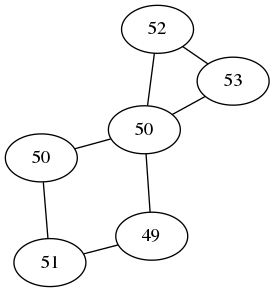
\includegraphics{graph3.png} &
	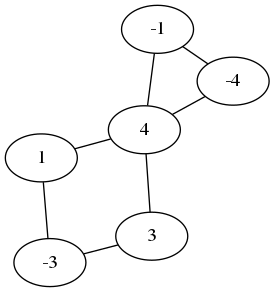
\includegraphics{graph4.png} \\
	The scalar field $u$ &
	The scalar field $\Delta u$
\end{tabular}
%SCRIPT echo 'graph { 1--2--4--5--6--4--3--1
%SCRIPT 1 [label="51"]
%SCRIPT 2 [label="49"]
%SCRIPT 3 [label="50"]
%SCRIPT 4 [label="50"]
%SCRIPT 5 [label="52"]
%SCRIPT 6 [label="53"]
%SCRIPT }' | neato -Tpng > graph3.png
%SCRIPT echo 'graph { 1--2--4--5--6--4--3--1
%SCRIPT 1 [label="-3"]
%SCRIPT 2 [label="3"]
%SCRIPT 3 [label="1"]
%SCRIPT 4 [label="4"]
%SCRIPT 5 [label="-1"]
%SCRIPT 6 [label="-4"]
%SCRIPT }' | neato -Tpng > graph4.png

Just from the definition, we can deduce several properties of the laplacian
\begin{enumerate}
	\item The sum of all the values of~$\Delta u$ is always zero
	\item If~$u(a)$ is a local maximum, then~$\Delta u(a)<0$
	\item If~$u(a)$ is a local minimum, then~$\Delta u(a)>0$
	\item If $u$ is constant, then~$\Delta u$ is zero
\end{enumerate}



If we fix an ordering of the vertices, then the scalar fields $u$ and $\Delta
u$ are two vectors in $\R^n$, and the linear operator $u\mapsto\Delta u$ is
given by the matrix $L=A-\mathtt{diag}(\mathtt{sum}(A))$.  This follows
directly by decomposing the definition of $\Delta$ into two sums:
\[
\Delta u(a)
=
\sum_{(a,b)\in E}
u(b)
-
\sum_{(a,b)\in E}
u(a)
=
-
u(a)\mathrm{degree}(a)
+\sum_{(a,b)\in E}
u(b)
\]


Notice that the Laplacian has a nice interpretation.
If we regard the values of $u$ as a quantity distributed on the vertices of
the graph, the condition $\Delta u = 0$ says that the quantity is distributed
evenly,  or in equilibrium: the amount of quantity at each vertex equals the
average amount over its neighbours.  In particular, if $u$ is constant then
$\Delta u = 0$.

Notice that the matrix~$L$ is always singular: a constant vector is an
eigenvector of eigenvalue 0.  If the graph has~$k$ connected components, then
we have null vectors that are constant on each connected component, thus the
matrix~$L$ has rank~$n-k$.


\subsection{Graph gradient and graph divergence}


Recall that scalar fields are functions defined on vertices and vector fields
are functions defined on edges.  Thus, the gradient transforms a function
defined on vertices into a function defined on edges.  There is a very
natural way of doing that: the value at each edge is obtained as the
difference between the values at each side of the edge.

\begin{tabular}{cc}
	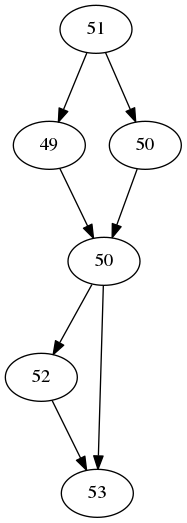
\includegraphics{graph5.png} &
	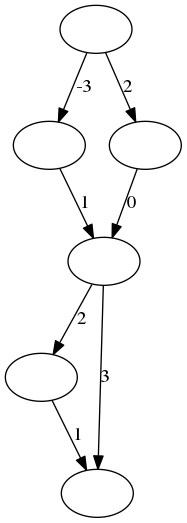
\includegraphics{graph6.png} \\
	The scalar field $u$ &
	The vector field $\nabla u$
\end{tabular}
%SCRIPT echo 'digraph {
%SCRIPT 1 [label="51"]
%SCRIPT 2 [label="49"]
%SCRIPT 3 [label="50"]
%SCRIPT 4 [label="50"]
%SCRIPT 5 [label="52"]
%SCRIPT 6 [label="53"]
%SCRIPT 1->2 [label=" "]
%SCRIPT 1->3 [label=" "]
%SCRIPT 2->4 [label=" "]
%SCRIPT 3->4 [label=" "]
%SCRIPT 4->5 [label=" "]
%SCRIPT 5->6 [label=" "]
%SCRIPT 4->6 [label=" "]
%SCRIPT }' | dot -Tpng > graph5.png
%SCRIPT echo 'digraph {
%SCRIPT 1 [label="  "]
%SCRIPT 2 [label="  "]
%SCRIPT 3 [label="  "]
%SCRIPT 4 [label="  "]
%SCRIPT 5 [label="  "]
%SCRIPT 6 [label="  "]
%SCRIPT 1->2 [label="-3"]
%SCRIPT 1->3 [label="2"]
%SCRIPT 2->4 [label="1"]
%SCRIPT 3->4 [label="0"]
%SCRIPT 4->5 [label="2"]
%SCRIPT 5->6 [label="1"]
%SCRIPT 4->6 [label="3"]
%SCRIPT  }' | dot -Tpng > graph6.png

More formally,  
let $G=(V,E)$ be a graph and $u:V\to\R$ be a scalar field.
The {\bf gradient} of $u$ is the vector field $\nabla u:E\to\R$ defined by
\[
\nabla u(a,b) := u(b) - u(a)
\qquad \mathrm{for}\ (a,b)\in E
\]
The matrix of this linear map is the incidence matrix $B$ of the graph.
Think of the gradient $\nabla u(a,b)$ as the directional derivative of $u$
at point $a$ in the direction of the vector from $a$ to $b$.



Now let $\mathbf{v}:E\to\R$ be a vector field.
The {\bf divergence} of $\mathbf{v}$ is the scalar field
$\mathrm{div}(\mathbf{v}):V\to\R$ defined by:
\[
\mathrm{div}(\mathbf{v})(a)
:=
\sum_{(a,b)\in E}\mathbf{v}(a,b)
-\sum_{(b,a)\in E}\mathbf{v}(b,a)
\qquad \mathrm{for}\ a\in V
\]
The matrix of this linear map is minus the transposed incidence matrix of the
graph $-B^T$.



Notice that the identity $\Delta=\mathrm{div\ grad}$ is trivial from the
definitions above, since both sides are exactly $\sum_{(a,b)\in E}u(b)-u(a)$.
Thus, $L=-B^TB$.


\subsection{Graph curl}


We do not need curls for our application, but let us say some words about
them.



These graph-theoretic analogues are easier to understand when we use
differential geometry instead of plain vector calculus.  In that case, the
discrete analogue of $k$-forms are functions defined over the $k$-cliques of the
graph.  Then the exterior derivative is readily built for all values of $k$,
and it contains the gradient, curl and divergence as particular cases.
The particularity of 3-dimensional manifolds comes from the fact that in
that in that case 1-forms and 2-forms have
the same dimension and can both be interpreted as ``vector fields'', thus the
curl operator is defined from the exterior derivative
$d:\Omega^1\to\Omega^2$.  In the case of graphs, we cannot in general identify functions
defined on edges to functions defined on triangles, except in one particular
case: when the graph is a triangulation.  In that case, there is a
construction that allows to define the curl of a vector field as a vector
field, by traversing the two triangles at each side of an edge.  The identity
$\mathrm{curl\ grad}=0$ is then the sum of 6 values that cancel pairwise, and
so on.  See the beautiful papers of Oliver Knill for a comprehensive coverage
of this.



\subsection{Graph subsets and their boundaries}


It is often necessary to deal with subset of graphs (for example, when we
want to interpolate a function which is known only over some vertices).
In order to do algebra with them, we model subsets as diagonal operators that
contain the indicator function of the subset as the diagonal entries.  This
model is used for subsets of vertices and subsets of edges.



{\bf Notations}:
Let $X=\{1,\ldots,n\}$ (or any finite ordered set) and $Y\subseteq X$.
Let $a$ be a vector of length $n$ and $A$ a
matrix of size $n\times n$ .  We use the following, somewhat ambiguous,
abuses of notation:

\begin{quotation}
$\mathrm{diag}(A)\in\R^n$:
the vector with the elements on the diagonal of $A$
$\mathrm{diag}(a)\in\R^{n\times n}$:
the diagonal matrix whose diagonal is $a$.
$\1_Y\in\R^{n}$: the indicator vector of the subset $Y$
$Y=\mathrm{diag}(\1_Y)\in\R^{n\times n}$: the diagonal operator of $Y$
\end{quotation}

This last notation is very convenient in image processing, because it
represents point-wise multiplication by a binary image as a linear operator
(with the same name as the binary image).  The $\mathrm{diag}$ operator has
the same semantics as that of octave/matlab.



Let $G=(V,E)$ be a graph with $n$ vertices and $m$ edges, and let
$\Omega\subseteq V$.
To avoid introducing new letters, we denote also by
$\Omega=\omega_{ij}$ the $n\times n$ matrix that contains the indicator
function of this set in its diagonal: $w_{ii}=1$ if $i\in V$ and $w_{jj}=0$
otherwise.
Notice that the matrix $I-\Omega$ corresponds to the
complementary set $\Omega^c$.



We define the {\bf boundary} of a subset of vertices $\Omega\subseteq V$ as
the subset of edges $\partial\Omega\subseteq E$ that go from $\Omega$ to
$\Omega^c$.  Notice that $\partial\Omega=E\cap(\Omega\times\Omega)$ in set
notation.  Since $\partial\Omega$ is a subset of edges, it corresponds to a
diagonal matrix, also named $\partial\Omega$, of size $m\times m$.
In matrix notation we have
\[\partial\Omega=\mathrm{diag}(B\mathrm{diag}(\Omega))\] where $B$ is the
incidence matrix of the graph.  We can also write
$\displaystyle\1_{\partial\Omega}=B\1_\Omega$.


\subsection{Equations on graphs}


Now that we have described the differential and boundary operators operator
in matrix form, it is immediate to write the discrete analogues of several
linear PDE.  This is very beautiful because the analytic properties of the
corresponding PDE are recovered by elementary linear algebra.



{\bf 3.6.1.}
{\bf Laplace} equation on the whole graph:
\[
Lu=0
\]
If the graph is connected, the matrix $L$ has rank $n-1$ thus its kernel is
one-dimensional, corresponding to the constant solutions $u=c$.



{\bf 3.6.2.}
{\bf Poisson} equation on the whole graph, with data $f:V\to\R$:
\[
Lu=f
\]
has a unique solution unless $f$ is constant.



{\bf 3.6.3.}
Laplace equation on a subset $\Omega\subseteq V$, with {\bf Dirichlet
boundary conditions}
$f:\Omega^c\to\R$:
\[
\Omega Lu + (I-\Omega)(u-f)=0
\]
Notice that this is written as an $n\times n$ linear system, but it has a
diagonal part corresponding to the values of $u$ outside of $\Omega$.
Notice also that the values of $f$ at the vertices that have no neighbors in
$\Omega$ only appear in the diagonal part.  The values of $f$ inside $\Omega$
do not appear at all (are cancelled out).



{\bf 3.6.4.}
Laplace equation on a subset $\Omega\subseteq V$,
with {\bf Neumann boundary conditions}
$g:\partial\Omega\to\R$:
\[
\Omega Lu + (\partial\Omega)(\nabla u - g)=0
\]
Or equivalently, by developing the boundary and gradient operators,
\[
\left[\Omega L + \mathrm{diag}(B\mathrm{diag}(\Omega))B\right]u =\mathrm{diag}(B\mathrm{diag}(\Omega)) g
\]
or, in an alternative notation
\[
(\mathrm{diag}(\1_\Omega) L + \mathrm{diag}(B\1_\Omega))B)u
=\mathrm{diag}(B\1_\Omega) g
\]



{\bf 3.6.5.}
{\bf Heat equation} on the whole graph with initial condition $u_0:V\to\R$:
\[
\begin{cases}
u_t & =Lu \\
u(0) & = u_0 
\end{cases}
\]
This is a system of $n$ first-order linear differential equations with
constant coefficients.  It has a closed-form solution using the matrix
exponential $u=e^{tL}u_0$.



{\bf 3.6.6.}
Heat equation with {\bf source term} $f:V\to\R$ and initial condition
$u_0:V\to\R$
\[
\begin{cases}
u_t & =Lu+f \\
u(0) & = u_0
\end{cases}
\]
It has likewise a closed-form solution $u=e^{tL}(u_0-L^{-1}f)-L^{-1}f$.
Notice that $L^{-1}f$ only makes sense when $f$ is not a constant vector.



{\bf 3.6.7.}
Other combinations are possible, and easy to deduce from the simpler cases:
Poisson and Heat equation on subsets with various boundary conditions, etc.



\subsection{Riemannian graph geometry}


The {\bf isotropic} case of ``anisotropic'' diffusion in image processing is
modelled by terms of the form $g\Delta u$, where $g$ is a positive-real valued
function on $\Omega$.  In the case of graphs, the function $g$ corresponds to
a scalar field $g:V\to\R$, which we associate to a diagonal $n\times n$
matrix $\tilde g$ with the values of $g$.  Then these terms become $\tilde gL
u$ in the corresponding discrete model.



Truly {\bf anisotropic} diffusion comes from terms of the form
$\mathrm{div}(D\nabla u)$, where the diffusivity $D$ is a field of
positive-definite symmetric matrices defined over $\Omega$.  In the case of
graphs, we have a matrix $\tilde D$, which is also diagonal, but now of
size $m\times m$.  Then these terms become $\mathrm{div}(D\nabla u)$ in the
discrete model.  Or, in matrix form, $B^TDBu$.


\subsection{Algebraic graph integral calculus}


Integral calculus can be generalized readily to graphs.  Integrals are
replaced by sums over a finite domain, and the various identities of integral
calculus (e.g., the divergence theorem) become immediate matrix identities.



Let $G=(V,E)$ be a graph with $V=\{1,\ldots,n\}$ and $E=\{1,\ldots,m\}$



Let $\Omega\subseteq V$ and let $f:V\to\R$ be a scalar field.
The {\bf integral} of $f$ over $\Omega$ is defined as
\[
\int_\Omega f=\sum_{p\in \Omega}f(p)
\]
in matrix notation we have
\(
\int_\Omega f := \mathrm{sum}(\Omega f).
\)
Notice that here $f$ is a vector of length $n$, $\Omega$ is an $n\times n$
matrix, and we are computing the sum of all the components of the vector
$\Omega f$ to obtain a single number.
Notice that $f$ must be defined everywhere, but only the values inside
$\Omega$ are used; thus, we could have defined $f$ only inside $\Omega$.



An {\bf interface} inside a graph  is defined as a set of edges $S\subseteq
E$.  Given a vector field $\mathbf{v}:E\to\R$ we define the {\bf flow}
of $\mathbf{v}$ through $S$
\[
\int_S \mathbf{v\cdot ds} := \sum_{e\in S}\mathbf{v}(e)
\]
or, in matrix notation, $\int_S \mathbf{v\cdot ds}=\mathrm{sum}(\tilde S
\mathbf{v})$ where $\tilde S$ is the diagonal matrix containing the indicator
function of $S$.
An interesting particular case happens when $S$ is the boundary of some
region $\Omega$.  We have seen above that the matrix $\tilde S$ is then
equal to $\mathrm{diag}(B\mathrm{diag}(\Omega))$.  This observation leads to the {\bf graph divergence
	theorem} that says that
\[
\int_{\partial\Omega} \mathbf{v\cdot ds} =\int_\Omega\mathrm{div}(\mathbf{v})
\]
or, in matrix notation,
\[
\1_\Omega\cdot(B^T\mathbf{v})
=
(B\1_\Omega)\cdot\mathbf{v}
\]
%\mathrm{sum}(\mathrm{diag}(B\mathrm{diag}(\Omega))\mathbf{v})
%=\mathrm{sum}(\Omega (B^T\mathbf{v}))
which is exactly the same thing, written differently.



